\documentclass{beamer}
% Use DS9 global theme
\usepackage{../../../shared/templates/ds9_theme}

% Title page configuration
\title[Kinematics in 2D]{PHYS12 CH3}
\subtitle{Kinematics in Two Dimensions}
\author[Mr. Gullo]{Mr. Gullo}
\date[Sept 2024]{September 2024}

% Table of contents at the beginning of each section
\AtBeginSection[]
{
  \begin{frame}
    \frametitle{Table of Contents}
    \tableofcontents[currentsection]
  \end{frame}
}

\begin{document}

% Title page
\frame{\titlepage}

% Table of contents
\begin{frame}
\frametitle{Table of Contents}
\tableofcontents
\end{frame}

\section{Introduction}

\begin{frame}
\frametitle{Introduction}
\begin{itemize}[<+->]
\item Kinematics in two dimensions
\item Vector addition and subtraction
\item Graphical and analytical methods
\item Projectile motion
\end{itemize}
\end{frame}

\section{Vectors and Scalars}

\begin{frame}
\frametitle{Vectors and Scalars}
\begin{columns}
\column{0.5\textwidth}
\begin{block}{Scalar Quantities}
\begin{itemize}
\item Have only magnitude
\item Examples: mass, temperature, time
\end{itemize}
\end{block}

\column{0.5\textwidth}
\begin{block}{Vector Quantities}
\begin{itemize}
\item Have magnitude and direction
\item Examples: displacement, velocity, acceleration
\end{itemize}
\end{block}
\end{columns}
\end{frame}

\section{Vector Addition and Subtraction: Graphical Methods}

\begin{frame}
\frametitle{Graphical Methods}
\begin{block}{Head-to-Tail Method}
\begin{enumerate}
\item Draw the first vector
\item Draw the second vector from the head of the first
\item Resultant vector: from tail of first to head of second
\end{enumerate}
\end{block}

\begin{block}{Parallelogram Method}
\begin{enumerate}
\item Draw both vectors from a common point
\item Complete the parallelogram
\item Resultant vector: diagonal of the parallelogram
\end{enumerate}
\end{block}
\end{frame}

\section{Vector Addition and Subtraction: Analytical Methods}

\begin{frame}
\frametitle{Trig Review}
\begin{columns}[T] % Top-aligned columns
    \column{0.48\textwidth}
    \begin{figure}
        \centering
        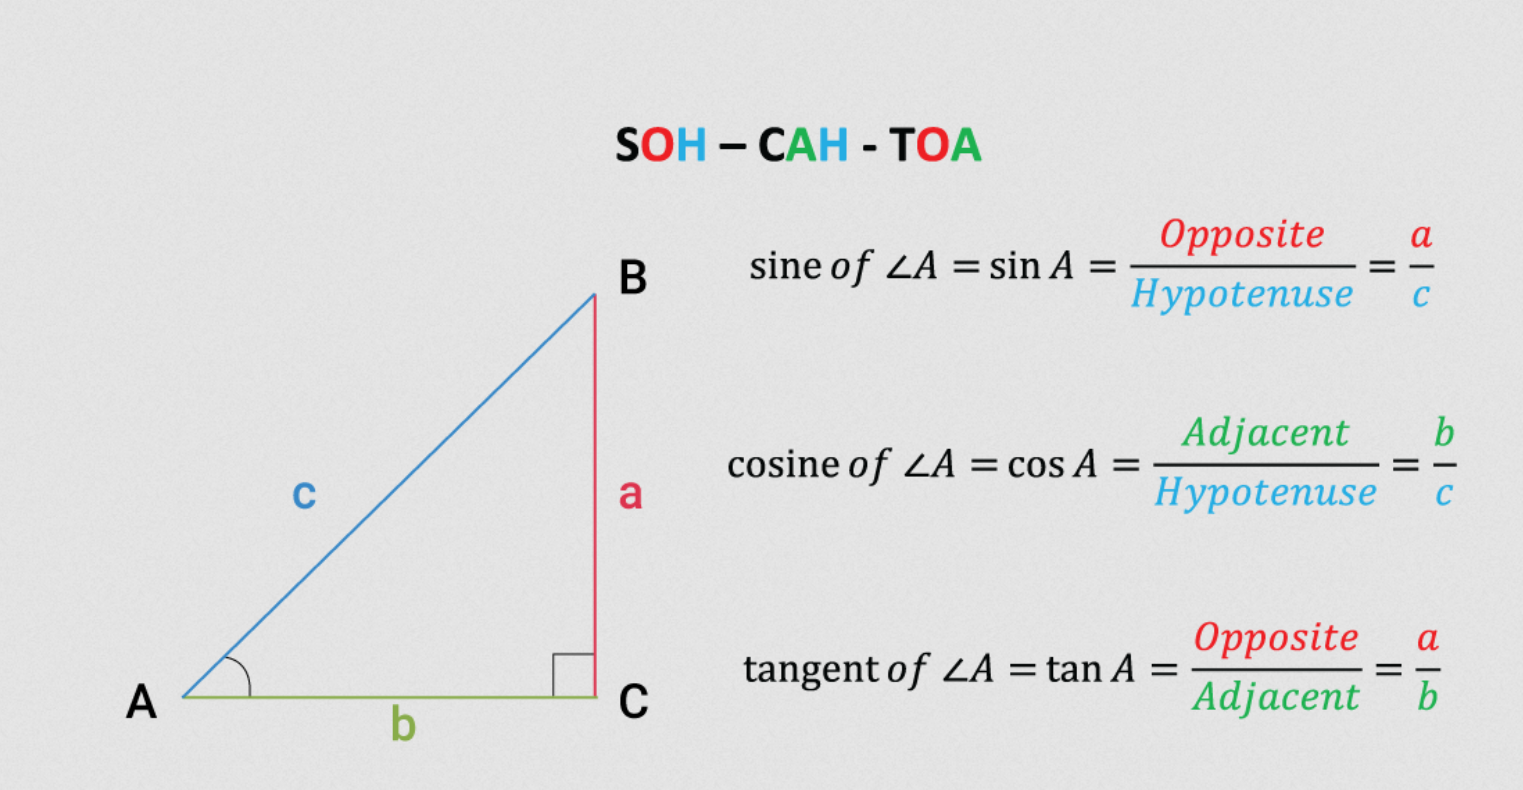
\includegraphics[width=\linewidth]{math-trigonometry-sohcahtoa.png}
        \caption{SOHCAHTOA mnemonic}
    \end{figure}

    \column{0.48\textwidth}
    \begin{figure}
        \centering
        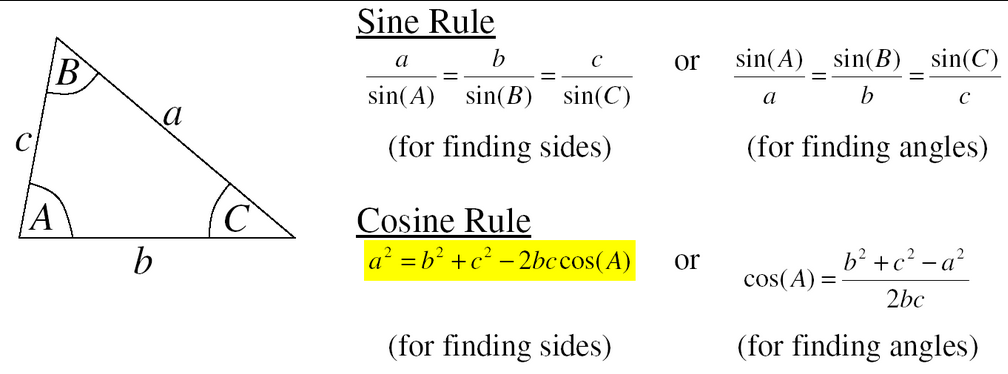
\includegraphics[width=\linewidth]{math-sine-cosine-laws.png}
        \caption{Sine and Cosine Laws}
    \end{figure}
\end{columns}
\end{frame}

\begin{frame}
\frametitle{Vector Components}
\begin{columns}
\column{0.6\textwidth}
Components of a vector $\vec{A}$:
\begin{align*}
A_x &= A \cos \theta \\
A_y &= A \sin \theta
\end{align*}
Where:
\begin{itemize}
\item $A$ is the magnitude of the vector
\item $\theta$ is the angle with the positive x-axis
\end{itemize}

\column{0.4\textwidth}
\begin{figure}
\centering
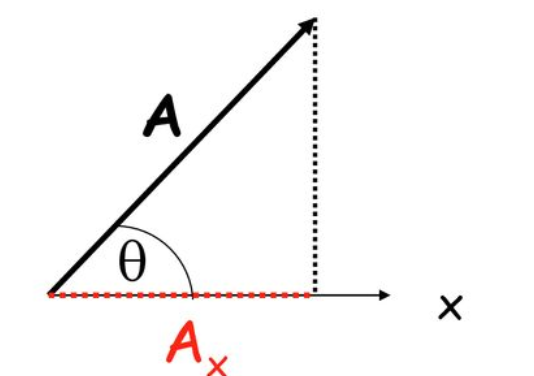
\includegraphics[width=0.8\textwidth]{phys12-vectors-vector-components.png}
\caption{Vector Components}
\end{figure}
\end{columns}
\end{frame}

\begin{frame}
\frametitle{Adding Vectors Analytically}
\begin{enumerate}[<+->]
\item Resolve vectors into x and y components
\item Sum x-components: $R_x = \sum A_x$
\item Sum y-components: $R_y = \sum A_y$
\item Find magnitude: $R = \sqrt{R_x^2 + R_y^2}$
\item Find direction: $\theta_R = \tan^{-1} \left( \frac{R_y}{R_x} \right)$
\end{enumerate}
\end{frame}

\section{Projectile Motion}

\begin{frame}
\frametitle{Projectile Motion}
\begin{block}{Assumptions}
\begin{itemize}
\item Air resistance is negligible
\item Acceleration due to gravity ($g$) is constant
\item Horizontal motion is at constant velocity
\end{itemize}
\end{block}

\begin{block}{Key Concepts}
\begin{itemize}
\item Two-dimensional motion
\item Vertical motion: accelerated
\item Horizontal motion: constant velocity
\end{itemize}
\end{block}
\end{frame}

\begin{frame}
\frametitle{Equations of Motion}
\begin{columns}
\column{0.5\textwidth}
Horizontal motion:
\begin{align*}
x &= v_{0x} t \\
v_x &= v_{0x}
\end{align*}

\column{0.5\textwidth}
Vertical motion:
\begin{align*}
y &= v_{0y} t - \frac{1}{2} g t^2 \\
v_y &= v_{0y} - g t
\end{align*}
\end{columns}

Where:
\begin{itemize}
\item $v_{0x} = v_0 \cos \theta$
\item $v_{0y} = v_0 \sin \theta$
\end{itemize}
\end{frame}

\begin{frame}
\frametitle{Range of a Projectile}
For a projectile launched and landing at the same vertical level:

\[
R = \frac{v_0^2 \sin 2\theta}{g}
\]

Where:
\begin{itemize}
\item $R$ is the range
\item $v_0$ is the initial velocity
\item $\theta$ is the launch angle
\item $g$ is the acceleration due to gravity
\end{itemize}
\end{frame}

\section{Worked Examples}

\begin{frame}
\frametitle{Example 1: Vector Addition}
Problem: Walk 18.0 m west, then 25.0 m north. Find distance and direction from start.

\begin{columns}
\column{0.6\textwidth}
Solution steps:
\begin{enumerate}
\item Resolve vectors into components
\item Sum components
\item Find magnitude of resultant
\item Find direction
\end{enumerate}

\column{0.4\textwidth}
\begin{figure}
\centering
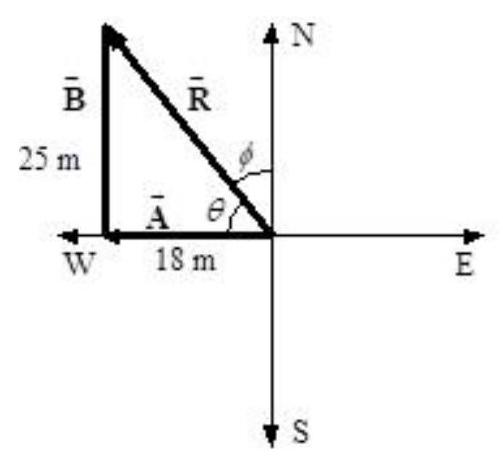
\includegraphics[width=0.8\textwidth]{phys12-vectors-vector-addition-figure-4.png}
\caption{Vector Addition}
\end{figure}
\end{columns}
\end{frame}

\begin{frame}
\frametitle{Example 1: Solution}
\begin{align*}
R_x &= -18.0 \text{ m} \\
R_y &= 25.0 \text{ m} \\
R &= \sqrt{(-18.0 \text{ m})^2 + (25.0 \text{ m})^2} = 30.8 \text{ m} \\
\theta &= \tan^{-1} \left( \frac{25.0}{-18.0} \right) = -54.25^\circ
\end{align*}

Answer: 30.8 m at $35.8^\circ$ west of north
\end{frame}

\begin{frame}
\frametitle{Example 2: Vector Components in Rotated Axes}
Problem: You fly 32.0 km in a straight line in still air in the direction $35.0^{\circ}$ south of west. \\
(a) Find the distances you would have to fly straight south and then straight west to arrive at the same point.
\\
\\

\\


\begin{align*}
D_W &= 32.0 \cos 35^\circ = 26.2 \text{ km} \\
D_S &= 32.0 \sin 35^\circ = 18.4 \text{ km}
\end{align*}

\end{frame}

\begin{frame}
\begin{columns}
\column{0.6\textwidth}
\frametitle{Example 2: Solution (continued)}
(b) Find the distances you would have to fly first in a direction $45.0^{\circ}$ south of west and then in a direction $45.0^{\circ}$ west of north. These are the components of the displacement along a different set of axes-one rotated $45^{\circ}$.
\begin{align*}
\theta' &= 35^\circ - 45^\circ = -10^\circ \\
D_{SW} &= 32.0 \cos 10^\circ = 31.5 \text{ km} \\
D_{NW} &= 32.0 \sin 10^\circ = 5.56 \text{ km}
\end{align*}

\column{0.4\textwidth}
\begin{figure}
\centering
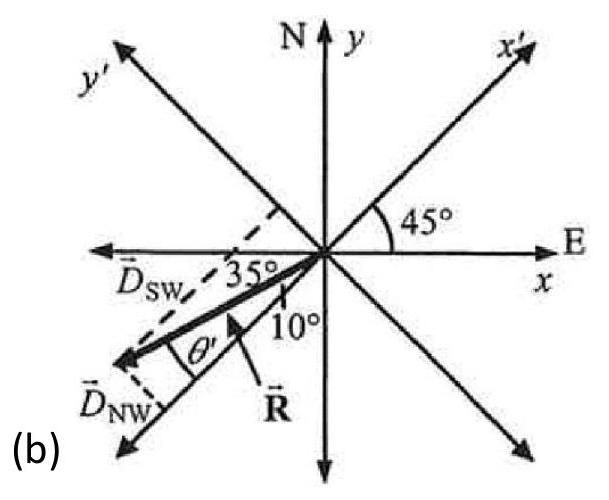
\includegraphics[width=0.8\textwidth]{phys12-vectors-vector-addition-figure-21.png}
\caption{Rotated Axes}
\end{figure}
\end{columns}

\end{frame}

\begin{frame}
\frametitle{Example 3: Vector Addition Verification}
Problem: Verify sum of vectors $\vec{A}$ (27.5 m at $66^\circ$ North of East) and $\vec{B}$ (30.0 m at $112^\circ$North of East)

\begin{columns}
\column{0.6\textwidth}
Steps:
\begin{enumerate}
\item Resolve vectors into components
\item Sum components
\item Find magnitude and direction of resultant
\end{enumerate}

\column{0.4\textwidth}
\begin{figure}
\centering
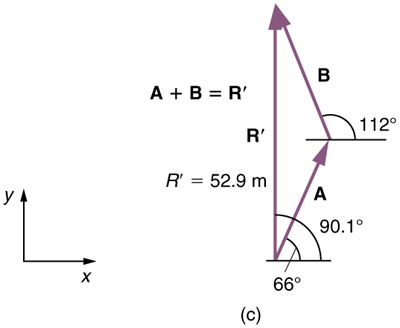
\includegraphics[width=0.8\textwidth]{phys12-vectors-vector-diagram-3-23.png}
\caption{Vector Addition}
\end{figure}
\end{columns}
\end{frame}

\begin{frame}
\frametitle{Example 3: Solution}
\begin{align*}
\text {Trigonometry is left as an exercise.} \\
R_x &= 11.19 \text{ m} + (-11.25 \text{ m}) = -0.06 \text{ m} \\
R_y &= 25.28 \text{ m} + 28.00 \text{ m} = 53.28 \text{ m} \\
R &= \sqrt{(-0.06 \text{ m})^2 + (53.28 \text{ m})^2} = 53.28 \text{ m} \\
\theta_R &= \tan^{-1} \left( \frac{53.28}{-0.06} \right) \approx -89.9^\circ
\end{align*}

Result: 53.28 m almost due north, slightly west
\end{frame}

\begin{frame}
\frametitle{Long Jump World Record Analysis}
Problem: The world long jump record is 8.95 m (Mike Powell, USA, 1991). Treated as a projectile, what is the maximum range obtainable by a person with a take-off speed of 9.5 m/s?

Assumptions:
\begin{itemize}
\item Scenario 1: Motion is on level ground (take-off and landing at same height)
\item Scenario 2: Person's center of mass is 1.0 m above the ground at take-off
\item Optimal angle is $45^\circ$
\item Air resistance is negligible
\end{itemize}
\end{frame}

\begin{frame}
\frametitle{Scenario 1: Level Ground}
Using the range formula:
\[
R = \frac{v_0^2 \sin 2\theta}{g} = \frac{(9.5 \text{ m/s})^2 \sin 90^\circ}{9.8 \text{ m/s}^2} = 9.21 \text{ m}
\]
\end{frame}

\begin{frame}
\frametitle{Scenario 2: 1.0 m Height Difference}
\begin{enumerate}
\item Find time of flight:
\[
y = -1.0 \text{ m} = (9.5 \text{ m/s})(\sin 45^\circ)t - \frac{1}{2}(9.80 \text{ m/s}^2)t^2
\]
Solving: $t = 1.51 \text{ s}$
\item Calculate range:
\[
R = v_0 (\cos 45^\circ) t = (9.5 \text{ m/s})(\cos 45^\circ)(1.51 \text{ s}) = 10.44 \text{ m}
\]
\end{enumerate}
\end{frame}

\begin{frame}
\frametitle{Conclusion}
Maximum obtainable range:
\begin{itemize}
\item Scenario 1 (level ground): 9.21 m
\item Scenario 2 (1.0 m height difference): 10.44 m
\end{itemize}
Both scenarios exceed the world record of 8.95 m, likely due to idealized assumptions.
\end{frame}
\section{Conclusion}

\begin{frame}
\frametitle{Conclusion}
\begin{itemize}[<+->]
\item Vectors are essential for describing motion in two dimensions
\item Both graphical and analytical methods are important
\item Projectile motion combines horizontal and vertical components
\item Practice problem-solving to master these concepts
\end{itemize}
\end{frame}

\end{document}